\subsubsection{Simple adder in SAT/SMT}

Let's solve the following equation $a+b=4 \equiv 2^4$ on the 4-bit CPU (hence, modulo $2^4$):

\lstinputlisting[style=customsmt]{\CURPATH/adder/bvadd_example.smt}

There are 16 possible solutions (easy to check even by hand):

\begin{lstlisting}
(model
	(define-fun a () (_ BitVec 4) (_ bv0 4)) ; 0x0
	(define-fun b () (_ BitVec 4) (_ bv4 4)) ; 0x4
)
(model
	(define-fun a () (_ BitVec 4) (_ bv12 4)) ; 0xc
	(define-fun b () (_ BitVec 4) (_ bv8 4)) ; 0x8
)

...

(model
	(define-fun a () (_ BitVec 4) (_ bv9 4)) ; 0x9
	(define-fun b () (_ BitVec 4) (_ bv11 4)) ; 0xb
)
Model count: 16
\end{lstlisting}

How I implemented this in my toy-level SMT solver?

First, we need an electronic adder, like it's implemented in digital circuits.
This is basic block (full-adder) (image taken from Wikipeda):

\begin{figure}[H]
\centering
\frame{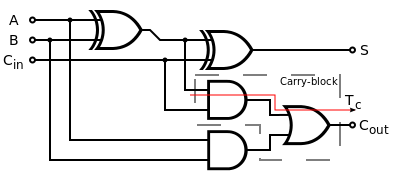
\includegraphics[scale=0.6]{\CURPATH/adder/400px-Full-adder_logic_diagram.svg.png}}
\end{figure}

This is how full adders gathered together to form a simple 4-bit carry-ripple adder (also from Wikipedia):

\begin{figure}[H]
\centering
\frame{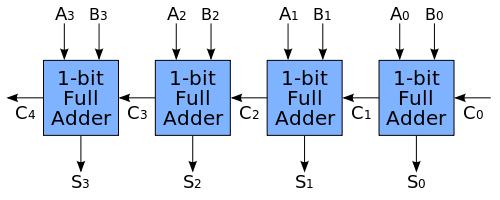
\includegraphics[scale=0.6]{\CURPATH/adder/500px-4-bit_ripple_carry_adder.svg.png}}
\end{figure}

More info from wikipedia: \url{https://en.wikipedia.org/wiki/Adder_(electronics)}.

I'm implementing full-adder like this:

\begin{lstlisting}
void add_Tseitin_XOR(int v1, int v2, int v3)
{
	add_comment ("%s %d=%d^%d", __FUNCTION__, v3, v1, v2);
	add_clause3 (-v1, -v2, -v3);
	add_clause3 (v1, v2, -v3);
	add_clause3 (v1, -v2, v3);
	add_clause3 (-v1, v2, v3);
};

void add_Tseitin_OR2(int v1, int v2, int var_out)
{
	add_comment ("%s %d=%d|%d", __FUNCTION__, var_out, v1, v2);
	add_clause("%d %d -%d", v1, v2, var_out);
	add_clause2(-v1, var_out);
	add_clause2(-v2, var_out);
};

void add_Tseitin_AND(int a, int b, int out)
{
	add_comment ("%s %d=%d&%d", __FUNCTION__, out, a, b);
	add_clause3 (-a, -b, out);
	add_clause2 (a, -out);
	add_clause2 (b, -out);
};

void add_FA(int a, int b, int cin, int s, int cout)
{
	add_comment("%s inputs=%d, %d, cin=%d, s=%d, cout=%d", __FUNCTION__, a, b, cin, s, cout);
	// allocate 3 "joint" variables:
	int XOR1_out=next_var_no++;
	int AND1_out=next_var_no++;
	int AND2_out=next_var_no++;
	// add gates and connect them.
	// order doesn't matter, BTW:
	add_Tseitin_XOR(a, b, XOR1_out);
	add_Tseitin_XOR(XOR1_out, cin, s);
	add_Tseitin_AND(XOR1_out, cin, AND1_out);
	add_Tseitin_AND(a, b, AND2_out);
	add_Tseitin_OR2(AND1_out, AND2_out, cout);
};
\end{lstlisting}

( \url{https://github.com/DennisYurichev/MK85/blob/master/MK85.cc} )

|add\_Tseitin*()| functions makes logic gates in CNF form: \url{https://en.wikipedia.org/wiki/Tseytin_transformation}.
Then I connect logic gates to make full-adder.

Then I connect full-adders to create a n-bit adder:

\begin{lstlisting}
void generate_adder(struct variable* a, struct variable* b, struct variable *carry_in, // inputs
	struct variable** sum, struct variable** carry_out) // outputs
{

	...

	*sum=create_internal_variable("adder_sum", TY_BITVEC, a->width);

	int carry=carry_in->var_no;

	// the first full-adder could be half-adder, but we make things simple here
	for (int i=0; i<a->width; i++)
	{
		*carry_out=create_internal_variable("adder_carry", TY_BOOL, 1);
		add_FA(a->var_no+i, b->var_no+i, carry, (*sum)->var_no+i, (*carry_out)->var_no);
		// newly created carry_out is a carry_in for the next full-adder:
		carry=(*carry_out)->var_no;
	};
};
\end{lstlisting}

( \url{https://github.com/DennisYurichev/MK85/blob/master/MK85.cc} )

Let's take a look on output CNF file:

\lstinputlisting{\CURPATH/adder/tmp.cnf}

Filter out comments:

\lstinputlisting{\CURPATH/adder/tmp.cnf.comments}

I make these functions add variable numbers to comments.
And you can see how all the signals are routed inside each full-adder.

|generate\_EQ()| function makes two bitvectors equal by XOR-ing two bitvectors.
Resulting bitvector is then OR-ed, and result must be zero.

% TODO \ref{}
Again, this SAT instance is small enough to be handled by my simple SAT backtracking solver:

\begin{lstlisting}
SAT
-1 2 -3 -4 -5 -6 -7 -8 9 -10 -11 -12 13 -14 -15 -16 -17 -18 -19 -20 -21 -22 -23 24 -25 -26 -27 -28 -29 -30 -31 -32 33 -34 -35 -36
-37 -38 -39 40 0
SAT
-1 2 -3 -4 -5 6 -7 -8 9 10 -11 -12 13 -14 -15 -16 -17 -18 -19 -20 -21 -22 -23 24 -25 -26 27 -28 -29 30 -31 -32 33 -34 -35 -36 -37
-38 -39 40 0

...

SAT
-1 2 3 4 5 -6 7 -8 9 10 -11 -12 13 -14 15 -16 -17 18 19 20 21 -22 23 -24 -25 26 27 28 29 -30 -31 -32 33 -34 -35 -36 -37 -38 -39 40 0
SAT
-1 2 3 4 5 6 7 -8 9 -10 -11 -12 13 -14 15 -16 -17 18 19 20 21 -22 23 -24 -25 26 27 28 29 -30 -31 -32 33 -34 -35 -36 -37 -38 -39 40 0
UNSAT
solutions= 16
\end{lstlisting}

%Another post in my blog where I write about adders in SAT: _HTML_LINK_AS_IS(`https://yurichev.com/blog/factor_SAT/').</p>

